% GuardedSOC -- a new paper, written from the evidence (2026-11-01, branch paper-v2; system name and result
% figures 2026-11-08, see RESEARCH_LOG.md). "AgentSOC" below means the base paper (Roy and Singh) only.
% Not derived from paper/agentsoc_combined.tex. Every number is taken from experiments/RESULTS.md; the section
% (C1-C5) is named in the text or the table caption. Claims follow experiments/PAPER_CLAIMS_TO_REVISE.md.
% Base-paper statements: Roy and Singh, ICAIC 2026, arXiv:2604.20134v1. Every number, with its RESULTS.md section
% or base-paper page: paper/agentsoc_v2_numbers.md. Authors and the repository link are TODOs.
\documentclass[conference]{IEEEtran}
\IEEEoverridecommandlockouts
\usepackage{cite}
\usepackage{amsmath,amssymb}
\usepackage{graphicx}
\usepackage{xcolor}
\usepackage{booktabs}
\usepackage{array}
\usepackage{url}
\usepackage{tikz}
\usepackage{pgfplots}
\pgfplotsset{compat=1.18}
\usetikzlibrary{arrows.meta,patterns}
\definecolor{ctrust}{HTML}{199E70}\definecolor{cllm}{HTML}{3987E5}\definecolor{ctext}{HTML}{D95926}
% Result figures, readable in grayscale: hatched = acting rule or no defence, solid = asymmetric trust or the
% defence, white = the reference condition. Every value printed on a bar is typed from experiments/RESULTS.md.
\pgfplotsset{
  actingbar/.style={draw=black, pattern=north east lines, pattern color=ctext!80!black},
  trustbar/.style={draw=black, fill=ctrust!55},
  basebar/.style={draw=black, fill=white},
}
\tikzset{val/.style={font=\scriptsize, inner sep=1.5pt}}   % a value printed on a bar (typed from RESULTS.md)
\newcommand{\todo}[1]{\textcolor{red}{[TODO: #1]}}

\begin{document}

\title{GuardedSOC: An Agentic SOC Tested Against\\Injected Log Text and Poisoned Memory}

\author{\IEEEauthorblockN{\todo{author names}}
\IEEEauthorblockA{\todo{affiliations and contact}}}

\maketitle

\begin{abstract}
Agentic designs for security operations centres (SOCs) put a large language model (LLM) and a learning knowledge
store into the triage loop. Both consume data an attacker can shape: the model reads log text, and the store adapts
to observed activity. AgentSOC, the framework we build on, was evaluated conceptually and on one proof-of-concept
incident, with no adversary aimed at either. We implement its loop end to end as GuardedSOC and add
a store that learns only through a learning gate, an analyst review loop with unlearning, fail-safe processing,
and asymmetric trust: the LLM's output may add review but cannot dismiss a case, start an automatic action or
teach the store. On 500 GUIDE v2 alert pairs, an undefended LLM agent was hijacked on 130/439 pairs, while the
pipeline's response was suppressed on 4/428; these are different measures. On 14 test days of DEDALE testbed logs,
learning the benign weeks cut host reviews from 6095.4 to 65.2 per day while the same 400 labelled attack events
still raised alerts. Under asymmetric trust, 0/72 attack cases were dismissed in E1 on DEDALE, whichever text the
attacker injected. Prompt-level defences were not tested as baselines.
\end{abstract}

\begin{IEEEkeywords}
security operations, agentic AI, prompt injection, memory poisoning, alert triage
\end{IEEEkeywords}

\section{Introduction}

Security operations centres (SOCs) receive far more alarms than analysts can examine, and most of those alarms
turn out to be harmless~\cite{alahmadi}. Agentic designs answer this by placing an LLM and a knowledge store inside
the triage loop. AgentSOC~\cite{agentsoc} is such a design: an LLM suggests how an incident might unfold, a graph
check removes suggestions the environment cannot support, a scoring module ranks responses, and a store keeps
enterprise context together with what earlier cycles observed.

Two parts of this arrangement read data the attacker can shape. The LLM reads free text from the logs: a command
line, a script block, a raw event record. Whoever runs a process on a monitored host chooses that text, and text
that reaches an LLM can redirect it~\cite{perez,greshake,liu}. The store adapts to what it observes, and a detector
that learns from observed traffic can be trained to accept an attack~\cite{antidote}; agent memories and retrieval
corpora share the weakness~\cite{agentpoison,poisonedrag}. The AgentSOC paper assumed an attacker who steals
credentials, moves laterally and escalates privileges, and it demonstrated the loop on a single proof-of-concept
incident~\cite{agentsoc}. That scope suits the introduction of an architecture. It leaves open what happens when
the attacker targets the model's input or the store's memory, and how the loop behaves over weeks of telemetry
with analysts in it.

We address these questions with a working system, GuardedSOC. GuardedSOC builds on and extends the AgentSOC
design~\cite{agentsoc}: it keeps the LLM hypothesis engine, the structural check and the response ranking inside a
perception--reasoning--action loop, and adds the defences and the evaluation described below. We make three
contributions:
\begin{enumerate}
\item An end-to-end implementation of the perception--reasoning--action loop, extended with a knowledge store that
learns benign behaviour only through a learning gate, an analyst inbox whose verdicts feed the store, and
unlearning once a host is confirmed compromised. We evaluate it on clean and contaminated alert pairs from GUIDE~v2
and on 14 test days of DEDALE testbed telemetry.
\item Measurements of both attack surfaces: text an attacker writes into logs (on GUIDE, and through the whole loop
on DEDALE), and poisoning of the learned memory, either by learning without a gate or through a misled analyst.
\item Asymmetric trust, a rule under which the LLM's output can add review but cannot dismiss a case, start an
automatic action or make anything learnable. It holds by construction for what the LLM's output can cause, and each
case can be checked, because the pipeline derives two decisions for every case, one that ignores the model and one
that uses it, and keeps the first unless the second asks for review. We combine it with fail-safe processing, so that input the
pipeline cannot handle leads to review rather than to a stalled loop.
\end{enumerate}
Section~\ref{sec:base} summarises the base paper and related work, Section~\ref{sec:system} describes the system,
Section~\ref{sec:setup} the evaluation setup and Section~\ref{sec:results} the results;
Section~\ref{sec:discussion} discusses them together with the limitations.

\section{Base Paper and Related Work}\label{sec:base}

\subsection{AgentSOC}
AgentSOC~\cite{agentsoc} arranges SOC automation as a perception layer, an agentic reasoning layer, an action and
playbook layer and an internal knowledge store, with real-time monitoring returning execution outcomes to the
store. The reasoning layer has three engines. The Narrative Counterfactual Engine (NCE) prompts an LLM for several
candidate attack progressions per incident, each tied to ATT\&CK techniques~\cite{attack} and given a confidence.
The Structural Simulation Engine (SSE) walks identity, privilege and network graphs and drops candidates whose
preconditions fail. RSEM, the Risk Scoring and Evaluation Module, orders candidate responses by a weighted
difference of containment value and business impact. Playbooks with a high projected impact go to analysts, execution begins
in dry-run mode with audit logs and rollback, and the store holds static enterprise context next to knowledge
derived from earlier cycles.

The base paper evaluates the design on a conceptual enterprise scenario and a proof of concept that used a
5,000-event sample of the LANL authentication data and a synthetic 50-node topology, with GPT-4 proposing the
hypotheses; its walk-through incident took about 506~ms end to end, 480~ms of it in the LLM~\cite{agentsoc}. The
authors list the fixed sample, the small topology, dry-run actions without feedback from live systems and
simplified business-impact scores as limitations, and name continuous telemetry and human-in-the-loop checkpoints
as future work. Three questions are open: whether data an attacker writes can steer the reasoning layer, whether
the store's learning can be turned against the defender, and how the loop behaves over time with analysts.
Table~\ref{tab:compare} sets the base design and this work side by side.

\begin{table*}[t]
\caption{AgentSOC~\cite{agentsoc} and this work. Base-paper entries come from its Sections III and IV; entries for
this work name the section of our results file (C1--C5).}
\label{tab:compare}
\centering\footnotesize
\begin{tabular}{@{}>{\raggedright}p{2.6cm}>{\raggedright}p{6.4cm}>{\raggedright\arraybackslash}p{7.6cm}@{}}
\toprule
Aspect & AgentSOC (base paper) & This work \\
\midrule
Attacker model & Steals credentials, moves laterally, escalates privileges; detecting zero-days and analysing
malware are out of scope & Adds an attacker who writes text into logs the LLM reads, and one who poisons the learned
memory (C1, C3) \\
Memory and learning & Store keeps enterprise context and knowledge updated from perception and action cycles &
Store learns benign patterns only through a learning gate; unlearning after a confirmed compromise (C2, C3) \\
Analyst loop & High-impact playbooks routed to analysts; human-in-the-loop checkpoints listed as future work &
Analyst inbox whose verdicts teach the store; response delays from 1 to 72 hours measured (C3, C5) \\
LLM output & SSE removes structurally infeasible hypotheses & Asymmetric trust: by construction, for what the LLM's
output can cause, the output can only add review (C1, C4) \\
Failure handling & Dry-run start, audit logs and rollback paths & This work adds: malformed events refused and
counted; failing events quarantined, with recovery from the last checkpoint; pipeline errors routed to review \\
Data & 5,000-event sample of LANL authentication logs; synthetic 50-node topology & GUIDE v2: 500 pairs for
development, 500 held out; DEDALE testbed host and network logs (C1, C2) \\
LLM & GPT-4 in the proof of concept & gemini-3.1-flash-lite; gpt-oss-20b on the GUIDE development pairs (C1) \\
Evaluation & Conceptual scenario and one proof-of-concept incident (about 506~ms end to end) & Paired contamination
tests; 14 test days under learning, analyst and LLM conditions; Wilson intervals and exact McNemar tests
(C1--C5) \\
\bottomrule
\end{tabular}
\end{table*}

\subsection{Related work}
Prompt injection was first shown with instructions written into the prompt itself~\cite{perez}, then indirectly,
through content that an LLM-integrated application retrieves~\cite{greshake}; Liu et al.\ formalise and benchmark
attacks and defences~\cite{liu}. Logs are content of that kind: the attacker produces them and the SOC's model
reads them. Defences at the prompt or model level mark untrusted input so the model can tell it apart
(spotlighting~\cite{spotlighting}) or train the model to follow only a separate instruction channel
(StruQ~\cite{struq}); they make the model follow injected text less often. CaMeL~\cite{camel} instead fixes, outside
the model, what untrusted data may influence. Asymmetric trust applies that second approach to a SOC: it does not
try to make the model resist, it limits what the model's output can change. Poisoning of learning detectors has a
long history~\cite{antidote}, and LLM agents inherit it through memories and retrieval
stores~\cite{agentpoison,poisonedrag}; we use a targeted form of unlearning~\cite{unlearning} as one remedy. Our
data come from GUIDE~\cite{guide}, Microsoft's incident-triage corpus, and DEDALE~\cite{dedale}, a labelled APT
dataset recorded on a testbed.

\section{System}\label{sec:system}

\begin{figure*}[!t]
\centering
\definecolor{csafe}{HTML}{7B4FB3}
\begin{tikzpicture}[font=\footnotesize, >={Stealth[length=1.6mm, width=1.3mm]},
  comp/.style={rounded corners=1.5pt, align=center, inner sep=2pt, anchor=north west, fill=white, draw=black!65,
    line width=0.5pt},
  trusted/.style={fill=ctrust!14, draw=ctrust!70!black, line width=0.6pt},
  attacker/.style={fill=ctext!17, draw=ctext!75!black, line width=1.4pt},
  llm/.style={fill=cllm!14, draw=cllm!75!black, double, double distance=0.9pt, line width=0.4pt},
  safety/.style={fill=csafe!12, draw=csafe!80!black, line width=1.1pt, dash pattern=on 4pt off 1.2pt on 1pt off 1.2pt},
  guideonly/.style={fill=white, draw=black!80, dashed, line width=0.5pt},
  layer/.style={rounded corners=3pt, fill=black!4, draw=black!45, line width=0.5pt},
  ltitle/.style={font=\footnotesize\bfseries, inner sep=3pt},
  flow/.style={->, line width=0.55pt, draw=black!80},
  both/.style={<->, line width=0.55pt, draw=black!80},
  lab/.style={font=\footnotesize, inner sep=1pt, align=center}]
% Routing columns and rows below the action layer.
\coordinate (dx) at (4.4,0); \coordinate (ex) at (6.0,0); \coordinate (rx) at (17.9,0);
\coordinate (dy) at (0,-8.42); \coordinate (ey) at (0,-8.17);
% ---------------- Perception Layer ----------------
\draw[layer] (0,0) rectangle (11.5,-2.0);
\node[ltitle, anchor=north west] at (0,0) {PERCEPTION LAYER};
\node[comp, text width=29mm, minimum height=14.5mm] (an) at (0.2,-0.42)
  {\textbf{Alert Normalization}\\splits each event into trusted fields and free text};
\node[comp, text width=32.5mm, minimum height=14.5mm] (sc) at (3.75,-0.42)
  {\textbf{Situational Contextualization}\\adds context from the store, keyed by trusted fields};
\node[comp, text width=35mm, minimum height=14.5mm] (nr) at (7.65,-0.42)
  {\textbf{Noise Reduction}\\detectors alert only on unlearned patterns; alerts sharing a pattern form a case};
\draw[flow] (3.26,-1.15) -- (3.75,-1.15);
\draw[flow] (7.16,-1.15) -- (7.65,-1.15);
% ---------------- Trusted fields | free text ----------------
\node[comp, trusted, text width=69.5mm, minimum height=7.8mm] (tf) at (0.2,-2.25)
  {\textbf{Trusted fields} (sensors, inventory): host, account, addresses, ports, event ids};
\node[comp, attacker, text width=35mm, minimum height=7.8mm] (ft) at (7.65,-2.25)
  {\textbf{Free text}, written by the attacker};
\draw[flow, draw=ctrust!70!black] (an.south) -- (an.south |- tf.north);
\draw[flow, draw=ctext!80!black] (nr.south) -- (nr.south |- ft.north);
% ---------------- Agentic Reasoning Layer ----------------
\draw[layer] (0,-3.18) rectangle (11.5,-5.76);
\node[ltitle, anchor=north west] at (0,-3.18) {AGENTIC REASONING LAYER};
\node[comp, text width=25mm, minimum height=11mm] (rsem) at (0.2,-3.6) {\textbf{RSEM (Rule Based)}\\ranks responses};
\node[comp, text width=27mm, minimum height=11mm] (sse) at (4.45,-3.6) {\textbf{SSE (Graph Based)}\\feasibility in the environment model};
\node[comp, llm, text width=23.5mm, minimum height=14.5mm] (nce) at (8.84,-3.6)
  {\textbf{NCE (LLM Based)}\\reads the first 512 characters of each free-text field};
\node[comp, guideonly, text width=36mm, minimum height=4.6mm] (guide) at (3.6,-4.83) {GUIDE only: ERA, destination check};
\draw[flow, draw=ctrust!70!black] (4.9,-3.03) -- (4.9,-3.6);
\node[lab, anchor=west, text=ctrust!60!black] at (4.98,-3.33) {model-free path};
\draw[flow, draw=ctext!80!black] (10.1,-3.03) -- (10.1,-3.6);
\draw[flow, draw=cllm!80!black] (8.84,-3.9) -- (7.31,-3.9) node[lab, midway, above] {Generate\\Hypothesis};
\draw[flow, draw=cllm!80!black] (7.31,-4.4) -- (8.84,-4.4) node[lab, midway, below] {Validate\\Possibility};
\draw[flow] (4.45,-4.35) -- (2.86,-4.35) node[lab, midway, above] {Published\\Attack Path};
\node[lab, anchor=north, text=cllm!70!black] at (10.09,-5.12) {model-assisted path};
% ---------------- Action and Playbook Layer ----------------
\draw[layer] (0,-5.91) rectangle (11.5,-7.92);
\node[ltitle, anchor=north east] at (11.5,-5.91) {ACTION AND PLAYBOOK LAYER};
\node[comp, text width=24mm, minimum height=14.8mm] (apg) at (0.2,-6.31)
  {\textbf{Adaptive Playbook Generator}\\builds playbooks from ranked actions};
\node[comp, safety, text width=49mm, minimum height=14.8mm] (guard) at (3.3,-6.31)
  {\textbf{Policy and Safety Guardrails}\\outcome = model-free decision, or review;\\a response only the model proposes waits for an analyst};
\node[comp, text width=22mm, minimum height=14.8mm] (exec) at (8.85,-6.31)
  {\textbf{Execution Interface}\\simulates model-free responses};
\draw[flow] (0.7,-4.7) -- (0.7,-6.31);
\node[lab, anchor=west] at (0.8,-5.3) {Ranked Actions};
\draw[flow] (guide.south) -- (guide.south |- guard.north);
\draw[flow] (2.76,-7.05) -- (3.3,-7.05);
\draw[flow] (8.36,-7.05) -- (8.85,-7.05);
% ---------------- Integrated Knowledge Store and Real-Time Monitoring ----------------
\node[comp, text width=15mm, minimum height=65mm, fill=black!7, draw=black!75, line width=0.9pt] (iks) at (13.0,0)
  {\textbf{Integrated Knowledge Store (IKS)}\\[3pt]learned patterns, environment model, enterprise context};
\draw[both] (11.5,-1.15) -- (13.0,-1.15) node[lab, midway, above] {learned\\patterns,\\context};
\draw[both] (11.5,-4.15) -- (13.0,-4.15) node[lab, midway, above] {environment\\model};
\draw[both] (11.5,-6.3) -- (13.0,-6.3) node[lab, midway, above] {enterprise\\context};
\node[comp, text width=15mm, minimum height=8.5mm] (rtm) at (13.0,-6.95) {\textbf{Real-Time Monitoring}};
\draw[both] (exec.east |- rtm.west) -- (rtm.west) node[lab, midway, above] {executed\\responses};
\draw[flow] (13.3,-6.95) -- (13.3,-6.5);
\node[lab, anchor=west] at (13.36,-6.72) {outcomes};
% ---------------- Legend, learning gate and analyst inbox ----------------
\begin{scope}[shift={(15.35,-0.05)}]
  \foreach \st/\lab/\y in {trusted/trusted data/0, attacker/attacker text/-0.36, llm/LLM-dependent/-0.72,
                          safety/safety control/-1.08, guideonly/GUIDE only/-1.44, comp/{other component}/-1.8}
    { \draw[\st, rounded corners=1pt] (0,\y) rectangle ++(0.42,-0.26);
      \node[lab, anchor=west] at (0.47,\y-0.13) {\lab}; }
\end{scope}
\node[comp, safety, text width=21mm, minimum height=14.8mm] (gate) at (15.35,-2.3)
  {\textbf{Learning gate}\\learns only cases dismissed without escalation};
\node[comp, text width=21mm, minimum height=22mm] (inbox) at (15.35,-3.98)
  {\textbf{Analyst inbox}\\human verdicts teach the store; a confirmed compromise triggers unlearning};
\draw[flow] (gate.west) -- (gate.west -| iks.east);
\draw[flow] (inbox.west) -- (inbox.west -| iks.east);
\draw[flow] (guard.south -| dx) |- (rx |- dy) |- (gate.east);
\node[lab, anchor=east] at (4.3,-8.2) {dismissed};
\draw[flow] (guard.south -| ex) |- (inbox.south |- ey) -- (inbox.south);
\node[lab, anchor=east] at (16.38,-7.25) {review and\\model-only\\proposals};
\end{tikzpicture}
\caption{GuardedSOC on the AgentSOC architecture~\cite{agentsoc}: the base design's layers, components and connections, with the security workflow this work adds marked by colour and outline. Program paths, though recorded by sensors, are chosen by the attacker for their own programs (Section~\ref{sec:system}-A). Entity binding checks the hosts and accounts in NCE's hypotheses against the trusted fields; SSE then marks each hypothesis feasible or infeasible (Validate Possibility), only feasible ones reach RSEM, and nothing is sent back to the LLM. On DEDALE the model-free path sends a case whose pattern the store has not learned to review. The model can raise the outcome to review but cannot lower it; responses of the model-free decision execute even when review is added. Analyst verdicts teach the store directly, and a confirmed compromise triggers unlearning.}
\label{fig:system}
\end{figure*}

\subsection{Pipeline}
Fig.~\ref{fig:system} shows GuardedSOC. Events from endpoint and network sensors are normalised and split into
two kinds of field. Structured fields (host, account, addresses, ports, event identifiers) come from sensors and
the asset inventory; we assume the attacker cannot alter them. Sensors also record program paths, the parent
program's included, but the attacker chooses the names and locations of their own programs, so these values can
influence which patterns the detectors see as new. Free text (command lines, script text, raw log records, process
and file names as strings) is whatever the attacker's activity produced, so the attacker controls it.

On host telemetry, detectors for new process lineage, named pipes, PowerShell activity, writes of executable
files, logons and access to the credential process compare each event's pattern with the knowledge store and raise
an alert when the pattern has not been learned. A pattern is built from sensor fields: hosts, accounts, program
paths, pipe names, written-file types, and for PowerShell a hash of the script text; alerts sharing a pattern form a case. For each case NCE asks the LLM
for ATT\&CK-labelled hypotheses, reading the first 512 characters of every free-text field. SSE checks each
hypothesis against the environment model, and entity binding flags a hypothesis whose host or account the
structured fields do not support. RSEM ranks responses, and guardrails decide which of them may run without an
analyst. On GUIDE a further component, ERA (evidence risk assessment), scans free text for injection-like content;
it can only escalate. Cases that need a person go to the analyst inbox, and an outcome monitor follows executed
responses.

\subsection{Asymmetric trust}
In our earlier runs NCE's hypotheses fed the decision directly; we call this the \emph{acting rule}. A hypothesis
judged infeasible could let a case be dismissed, and one that survived could lead to an automatic response within
the guardrails. Asymmetric trust replaces it with two decisions per case. The \emph{model-free decision} uses
everything except the LLM's output. On DEDALE that is the structured fields and the store, and a case whose pattern
the store has not learned goes to review (the rule for unreasoned cases); on GUIDE it also includes ERA and the
check of destination telemetry.
The \emph{model-assisted decision} adds NCE's hypotheses. The outcome is the model-free decision, unless the
model-assisted decision asks for review, in which case the outcome is review. Responses of the model-free decision
run automatically even when review is added; a response that only the model-assisted decision proposes waits for
an analyst. Only dismissed cases can be learned, and only the model-free decision can dismiss.

So, by construction for what the LLM's output can cause, the model cannot dismiss a case, trigger an automatic
response or teach the store; at most it adds a review. The rule covers nothing an analyst decides after reading
attacker text, and nothing about tampered sensor fields. Since it compares two decisions, it is easy to verify: our
tests replay recorded model answers and randomly generated adversarial hypotheses and check that no outcome is
less strict than the model-free decision.

\subsection{Learning gate and unlearning}
The store learns a case's pattern only when the case was dismissed without any escalation, and only 24 hours after
the case closed; if a case on the same host (for network alerts, the same endpoints) was escalated after this case
opened, the case is not learned at all. Under asymmetric trust
that means dismissed by the model-free decision, so neither attacker text nor the model can open the gate. Analyst
verdicts are the deliberate exception: a benign verdict teaches the store directly, which is how feedback lowers
the workload. When an analyst confirms a host as compromised, the store retracts what it recently learned on that
host and learns nothing further there.

\subsection{Fail-safe processing}
A loop that an input can stall serves the attacker as well as a loop that an input can fool. Malformed events are
refused and counted instead of being passed on. An event on which the pipeline fails is moved to a quarantine file,
and the live runner restores its last checkpoint and carries on; before this change such an event ended the loop.
An error inside triage sends the case to review instead of dropping it, and analyst commands are applied
atomically, so a failing command leaves no partial change. Checkpoints are signed and loaded through an allow-list
of classes. A check that scans evidence text for command-and-control indicators reads only the part of each field
the LLM was shown, which bounds its running time on long crafted text. These mechanisms are covered by unit tests,
not evaluated on a dataset; in the 43 replays behind our results no event was refused. The quarantine and the
recovery from a checkpoint belong to the live server; the experiment replays run the loop directly.

\section{Evaluation Setup}\label{sec:setup}

\subsection{GUIDE v2: contaminated alert pairs}
From GUIDE~\cite{guide} we built pairs of alerts that differ at a single injection site: a clean alert and a
contaminated twin carrying an attacker payload, with 500 pairs for development and 500 held out (C1). Entities, evidence
text and payloads are synthetic. GUIDE alerts run through the single-alert pipeline without a learned store, so
NCE's hypotheses are what raise a response there. A pair is \emph{suppressed} when the clean alert received a
response (review or an automatic response) and its twin did not. We compare suppressed pairs with flips in the
opposite direction using an exact McNemar test, keeping apart the flips caused by ERA's escalation, which are the
defence reacting; proportions carry 95\% Wilson intervals. The undefended comparison agent is the same model,
prompted with the alert's fields to return a verdict; it is \emph{hijacked} when it does not dismiss the clean
alert but dismisses the twin. Suppression concerns the pipeline's decision and hijacking the agent's own verdict, so the two
are different measures. We also count \emph{automatic containments removed}: pairs whose clean alert runs an
automatic block the trusted telemetry supports while the twin does not.

\subsection{DEDALE: weeks of testbed telemetry}
DEDALE~\cite{dedale} records an emulated small company over several weeks, including one multi-step attack; exact
labels exist for the events of the 2 attacked Windows clients. The store learns from the two benign weeks, and the
14 test days that follow are replayed in order, with host logs and network (Suricata) alerts (C2). A simulated
analyst answers from the labels after a set delay, optionally with reproducible mistakes. In experiment E1 the
attacker appends text to the command lines of their own processes: a routine-maintenance claim, a fake SOC
approval, or a request to isolate the domain controller instead; 84 events carry it, and in 38 cases the first
alert does (C1).

\subsection{Recorded answers, two rules, frozen results}
Every LLM answer was recorded once (gemini-3.1-flash-lite on both datasets, gpt-oss-20b on the GUIDE development
pairs) and is replayed, so no experiment needs a model call to reproduce. Each condition is a deterministic
replay. One script rebuilds our results file from the frozen score files in the repository, the GUIDE re-scoring
of the recorded answers and the replays' outputs in the DEDALE data folder, so a rebuild needs that data folder as
well as the repository; every number below is taken from that file, and we name its section (C1--C5). The acting rule and asymmetric trust are scored on the same recorded
answers. The asymmetric-trust numbers are the rows marked as such in sections C1 and C4 of the results file.

\section{Results}\label{sec:results}

\subsection{C1: text written into logs}
On GUIDE, contamination suppressed the pipeline's response on 4 of 428 development pairs whose clean alert was
answered (0.9\%, 95\% CI 0.4\%--2.4\%), on 3 of 437 held-out pairs (0.7\%, 0.2\%--2.0\%), and on 10 of 437
development pairs when gpt-oss-20b produced the hypotheses (2.3\%, 1.2\%--4.2\%). Against the flips in the other direction not caused by ERA, McNemar
gives $p=1$, $0.25$ and $0.3$: no detectable effect. ERA's escalation produced the opposite flip in 12, 10 and 12
pairs. No steered hypothesis led to an executed action; 7, 2 and 3 were held for an analyst. The undefended agent
was hijacked on 130 of 439 pairs (29.6\%, 25.5\%--34.0\%, $p=6.5\times10^{-17}$). In E1 on DEDALE, under the acting
rule and without an analyst, the maintenance text caused 1 dismissal among the 72 attack cases, the approval text 3
and the steering text 1; with an analyst, there were none (Fig.~\ref{fig:text}, left). In every E1 run the store learned no attack pattern and the same 400
labelled attack events raised alerts. The steering text did reach the model: NCE named the steered host in 30 of
38 injected cases (32 of 38 with the analyst), entity binding flagged every steered hypothesis (49 of 49 and 59 of
59), and no containment targeted that host.

\begin{figure}[t]
\centering
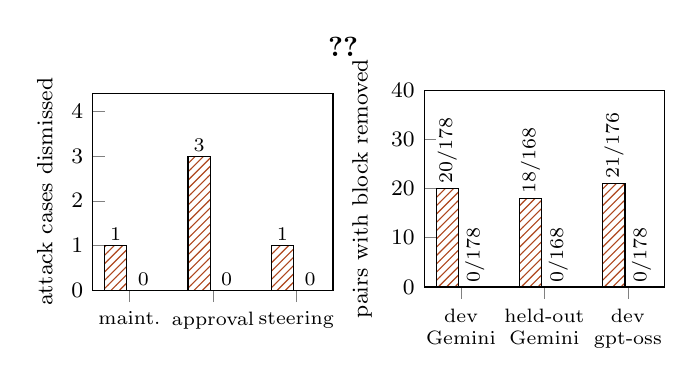
\begin{tikzpicture}
\pgfplotsset{twin/.style={ybar, bar width=8pt, scale only axis, width=3.05cm, height=2.5cm, ymin=0, tick pos=left,
  font=\footnotesize, xticklabel style={font=\scriptsize, align=center}}}
\begin{axis}[twin, name=e1, symbolic x coords={maint,appr,steer}, xtick={maint,appr,steer},
  xticklabels={{maint.},{approval},{steering}}, enlarge x limits=0.22, ymax=4.4,
  ylabel={attack cases dismissed}, legend to name=textlegend, legend columns=2,
  legend style={font=\scriptsize, draw=none, /tikz/every even column/.append style={column sep=6pt}}]
\addplot[actingbar, bar shift=-5pt] coordinates {(maint,1) (appr,3) (steer,1)};
\addlegendentry{acting rule}
\addplot[trustbar, bar shift=5pt] coordinates {(maint,0) (appr,0) (steer,0)};
\addlegendentry{asymmetric trust}
\node[val, above] at ([xshift=-5pt]axis cs:maint,1) {1};
\node[val, above] at ([xshift=-5pt]axis cs:appr,3) {3};
\node[val, above] at ([xshift=-5pt]axis cs:steer,1) {1};
\node[val, above] at ([xshift=5pt]axis cs:maint,0) {0};
\node[val, above] at ([xshift=5pt]axis cs:appr,0) {0};
\node[val, above] at ([xshift=5pt]axis cs:steer,0) {0};
\end{axis}
\begin{axis}[twin, at={(e1.outer east)}, anchor=outer west, symbolic x coords={gdev,ghold,odev},
  xtick={gdev,ghold,odev}, xticklabels={{dev\\Gemini},{held-out\\Gemini},{dev\\gpt-oss}},
  enlarge x limits=0.22, ymax=40, ylabel={pairs with block removed}]
\addplot[actingbar, bar shift=-5pt] coordinates {(gdev,20) (ghold,18) (odev,21)};
\addplot[trustbar, bar shift=5pt] coordinates {(gdev,0) (ghold,0) (odev,0)};
\node[val, rotate=90, anchor=west] at ([xshift=-5pt]axis cs:gdev,20) {20/178};
\node[val, rotate=90, anchor=west] at ([xshift=-5pt]axis cs:ghold,18) {18/168};
\node[val, rotate=90, anchor=west] at ([xshift=-5pt]axis cs:odev,21) {21/176};
\node[val, rotate=90, anchor=west] at ([xshift=5pt]axis cs:gdev,0) {0/178};
\node[val, rotate=90, anchor=west] at ([xshift=5pt]axis cs:ghold,0) {0/168};
\node[val, rotate=90, anchor=west] at ([xshift=5pt]axis cs:odev,0) {0/178};
\end{axis}
\node[anchor=south] at ([yshift=1pt]e1.outer north east) {\ref{textlegend}};
\end{tikzpicture}
\caption{Attacker-written text under the acting rule (hatched) and asymmetric trust (solid); C1 of the results
file, its asymmetric-trust rows for the solid bars. Left: attack cases (of 72) dismissed in E1 on DEDALE without an
analyst, per injected text (routine-maintenance claim, fake approval, steering). Right: GUIDE pairs in which
contamination removed an automatic block (gpt-oss: gpt-oss-20b); labels give the count over the pairs whose clean
alert executed one.}
\label{fig:text}
\end{figure}

\begin{table}[t]
\caption{Attacker-written text under the acting rule and under asymmetric trust (C1; asymmetric-trust rows of C1).
GUIDE: pairs; E1 on DEDALE: attack cases. No steered action was executed in any run.}
\label{tab:text}
\centering\footnotesize
\setlength{\tabcolsep}{3pt}
\resizebox{\columnwidth}{!}{%
\begin{tabular}{@{}llrr@{}}
\toprule
Setting & Measure & Acting rule & Asym.\ trust \\
\midrule
GUIDE dev, Gemini & suppressed & 4/428 & 4/428 \\
 & containments removed & 20/178 & 0/178 \\
GUIDE held-out, Gemini & suppressed & 3/437 & 3/437 \\
 & containments removed & 18/168 & 0/168 \\
GUIDE dev, gpt-oss-20b & suppressed & 10/437 & 10/437 \\
 & containments removed & 21/176 & 0/178 \\
\midrule
E1 on DEDALE, & dismissed, maintenance & 1/72 & 0/72 \\
no analyst & dismissed, approval & 3/72 & 0/72 \\
 & dismissed, steering & 1/72 & 0/72 \\
 & reviews per day, clean & 54.8 & 65.2 \\
E1 on DEDALE, & dismissed, each text & 0/72 & 0/72 \\
analyst (4 h) & reviews per day, clean & 33.2 & 34.1 \\
\bottomrule
\end{tabular}}
\end{table}

\subsection{C2: learning behind a gate}

\begin{figure}[t]
\centering
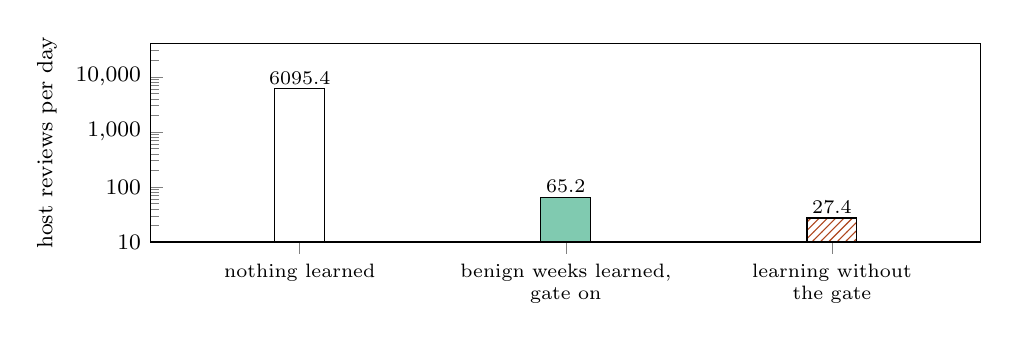
\begin{tikzpicture}
\begin{axis}[ybar, bar width=18pt, ymode=log, log origin=infty, ymin=10, ymax=40000, log ticks with fixed point,
  width=\columnwidth, height=4.1cm, symbolic x coords={none,gate,nogate}, xtick={none,gate,nogate},
  xticklabels={{nothing learned},{benign weeks learned,\\gate on},{learning without\\the gate}},
  xticklabel style={font=\scriptsize, align=center}, enlarge x limits=0.28, font=\footnotesize, tick pos=left,
  ylabel={host reviews per day}]
\addplot[basebar, bar shift=0pt] coordinates {(none,6095.4)};
\addplot[trustbar, bar shift=0pt] coordinates {(gate,65.2)};
\addplot[actingbar, bar shift=0pt] coordinates {(nogate,27.4)};
\node[val, above] at (axis cs:none,6095.4) {6095.4};
\node[val, above] at (axis cs:gate,65.2) {65.2};
\node[val, above] at (axis cs:nogate,27.4) {27.4};
\end{axis}
\end{tikzpicture}
\caption{Host reviews per day on DEDALE, log scale (C2). Learning without the gate has the fewest reviews only
because the store learned 38 attack cases' patterns as routine: 99 labelled attack events alerted, against 400 with
the gate.}
\label{fig:c2}
\end{figure}

With nothing learned, the host detectors produced 6095.4 reviews per day over 85336 test cases, raising 80
malicious cases and 473 labelled attack events (C2, Fig.~\ref{fig:c2}). After learning the benign weeks, reviews fell to 65.2 per day
over 913 cases; 72 malicious cases were raised, every one reviewed, and 400 labelled attack events alerted.
Continuing to learn behind the gate gave the same numbers: with neither NCE nor an analyst, no case is dismissed,
so the gate admits nothing new, and the reduction is due to the training weeks rather than to the gate. Learning
without the gate is where the memory turns against the defender. Reviews dropped to 27.4 per day, but the store
absorbed 38 attack cases' patterns as routine, only 38 malicious cases were raised, and 99 attack events alerted.
Network alerts followed the same pattern: 552.3 reviews per day with nothing learned, 26.1 after learning, and
without the gate 20.6, with 1 attack pattern learned.

\subsection{C3: poisoning through the analyst}

\begin{figure}[t]
\centering
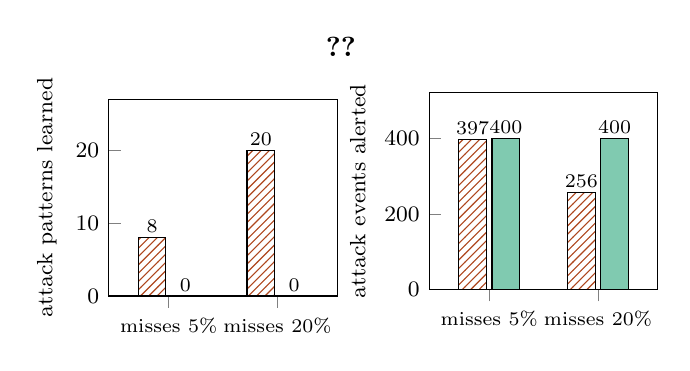
\begin{tikzpicture}
\pgfplotsset{poison/.style={ybar, bar width=10pt, scale only axis, width=2.9cm, height=2.5cm, ymin=0, tick pos=left,
  symbolic x coords={m5,m20}, xtick={m5,m20}, xticklabels={{misses 5\%},{misses 20\%}}, enlarge x limits=0.55,
  font=\footnotesize, xticklabel style={font=\scriptsize}}}
\begin{axis}[poison, name=learned, ymax=27, ylabel={attack patterns learned},
  legend to name=poisonlegend, legend columns=2,
  legend style={font=\scriptsize, draw=none, /tikz/every even column/.append style={column sep=6pt}}]
\addplot[actingbar, bar shift=-6pt] coordinates {(m5,8) (m20,20)};
\addlegendentry{without unlearning}
\addplot[trustbar, bar shift=6pt] coordinates {(m5,0) (m20,0)};
\addlegendentry{with unlearning}
\node[val, above] at ([xshift=-6pt]axis cs:m5,8) {8};
\node[val, above] at ([xshift=-6pt]axis cs:m20,20) {20};
\node[val, above] at ([xshift=6pt]axis cs:m5,0) {0};
\node[val, above] at ([xshift=6pt]axis cs:m20,0) {0};
\end{axis}
\begin{axis}[poison, at={(learned.outer east)}, anchor=outer west, ymax=520,
  ylabel={attack events alerted}]
\addplot[actingbar, bar shift=-6pt] coordinates {(m5,397) (m20,256)};
\addplot[trustbar, bar shift=6pt] coordinates {(m5,400) (m20,400)};
\node[val, above] at ([xshift=-6pt]axis cs:m5,397) {397};
\node[val, above] at ([xshift=-6pt]axis cs:m20,256) {256};
\node[val, above] at ([xshift=6pt]axis cs:m5,400) {400};
\node[val, above] at ([xshift=6pt]axis cs:m20,400) {400};
\end{axis}
\node[anchor=south] at ([yshift=1pt]learned.outer north east) {\ref{poisonlegend}};
\end{tikzpicture}
\caption{Poisoning through a simulated analyst who misses 5\% or 20\% of attacks (C3): attack cases' patterns
learned as routine (left) and labelled attack events alerted (right), without unlearning (hatched) and with
unlearning on confirmed compromise (solid).}
\label{fig:c3}
\end{figure}

The gate does not apply to analysts, so we simulated one who misses attacks (C3, Fig.~\ref{fig:c3}). Missing 5\% let the store learn 8
attack cases' patterns and left 397 events alerting; missing 20\% taught it 20 patterns and reduced the malicious
cases raised to 61 and the alerting events to 256, at 30.1 reviews per day. With unlearning on confirmed
compromise, both mistake rates
ended with 0 patterns learned, 72 malicious cases raised and 400 events alerting. The price is review load: 34.1
instead of 30.9 reviews per day with an analyst who is always right, and 44.6 instead of 31.4 with one who raises
5\% false alarms, since every false confirmation retracts benign learning.

\begin{table}[t]
\caption{DEDALE host logs, 14 test days. Top: learning and poisoning (C2, C3); bottom: the LLM (C4; the
asymmetric-trust rows of C4). Patterns: attack cases' patterns learned as routine.}
\label{tab:dedale}
\centering\footnotesize
\setlength{\tabcolsep}{3pt}
\resizebox{\columnwidth}{!}{%
\begin{tabular}{@{}lrrrr@{}}
\toprule
Condition & Reviews/day & Malicious raised & Events alerted & Patterns \\
\midrule
Nothing learned & 6095.4 & 80 & 473 & 0 \\
Benign weeks learned, gate & 65.2 & 72 & 400 & 0 \\
Learning without the gate & 27.4 & 38 & 99 & 38 \\
Analyst misses 20\% & 30.1 & 61 & 256 & 20 \\
\quad with unlearning & 34.1 & 72 & 400 & 0 \\
\midrule
 & Reviews/day & Malicious dism. & Benign dism. & \\
\midrule
NCE, closed world & 54.6 & 2/72 & 89 & \\
NCE, open world & 54.8 & 0/72 & 89 & \\
NCE and analyst & 33.2 & 0/72 & 30 & \\
NCE, asymmetric trust & 65.2 & 0/72 & 0 & \\
NCE and analyst, asym.\ trust & 34.1 & 0/72 & 0 & \\
\bottomrule
\end{tabular}}
\end{table}

\subsection{C4: the LLM on testbed telemetry}

\begin{figure}[t]
\centering
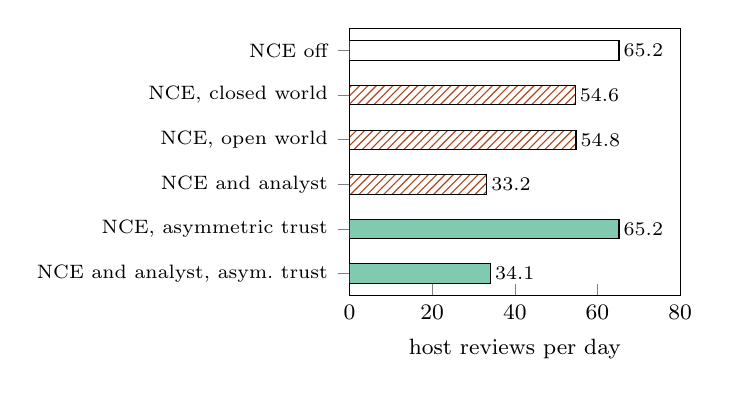
\begin{tikzpicture}
\begin{axis}[xbar, bar width=7pt, scale only axis, width=4.2cm, height=3.4cm, xmin=0, xmax=80,
  symbolic y coords={off,closed,open,ana,asym,asyman}, ytick={off,closed,open,ana,asym,asyman},
  yticklabels={{NCE off},{NCE, closed world},{NCE, open world},{NCE and analyst},{NCE, asymmetric trust},
  {NCE and analyst, asym.\ trust}}, y dir=reverse, enlarge y limits=0.1, font=\footnotesize, tick pos=left,
  yticklabel style={font=\scriptsize}, xlabel={host reviews per day}]
\addplot[basebar, bar shift=0pt] coordinates {(65.2,off)};
\addplot[actingbar, bar shift=0pt] coordinates {(54.6,closed) (54.8,open) (33.2,ana)};
\addplot[trustbar, bar shift=0pt] coordinates {(65.2,asym) (34.1,asyman)};
\node[val, right] at (axis cs:65.2,off) {65.2};
\node[val, right] at (axis cs:54.6,closed) {54.6};
\node[val, right] at (axis cs:54.8,open) {54.8};
\node[val, right] at (axis cs:33.2,ana) {33.2};
\node[val, right] at (axis cs:65.2,asym) {65.2};
\node[val, right] at (axis cs:34.1,asyman) {34.1};
\end{axis}
\end{tikzpicture}
\caption{Host reviews per day with the LLM (C4): NCE off (white), the acting rule (hatched) and asymmetric trust
(solid; the asymmetric-trust rows of C4). The closed-world run dismissed 2 of 72 malicious cases; the other runs
dismissed none of them.}
\label{fig:c4}
\end{figure}

Adding NCE under the acting rule with a closed-world feasibility check lowered reviews from 65.2 to 54.6 per day,
but dismissed 2 of 72 malicious cases together with 89 benign ones (C4, Fig.~\ref{fig:c4}). Both misses involved a server without
telemetry in the store, whose absence was read as impossibility. Treating unmonitored hosts as unknown (open world)
dismissed none of the 72 malicious cases and 89 benign ones, at 54.8 reviews per day; we adopted this rule after
seeing the misses, on the same data. With an analyst as well, NCE brought reviews to 33.2 per day against 34.1 for
the same analyst without NCE (C3), dismissing 30 benign cases. The workload NCE saves comes entirely from dismissing
cases, the same route the attacker used in E1. Each free-text field reaches the model cut to its first 512
characters; the command line exceeds that length in 1 of 797 first alerts, the raw log line in 718 of 856.

\subsection{C5: running the analyst loop}
Analyst feedback lowers the load further, and its delay matters (Fig.~\ref{fig:delay}, C5): 33.1, 34.1, 38.1 and
51.5 reviews per day with answers after 1, 4, 24 and 72 hours, against 65.2 without an analyst, with 72 malicious
cases raised and the same 400 events alerting at every delay. On the network side the attacker's server was
contained after 60, 240, 1440 and 4320 minutes, the analyst's delay in each case, and never without an analyst.
With a 4-hour analyst every stage of the attack reached review: initial access on client 2 first after 1.2
minutes (20 cases), lateral movement to client 1 after 28.5 (11), collection from the internal server after 30.0
(11) and exfiltration after 1265.0 minutes (4). With 5\% false alarms on the network side, approved blocks would
have hit benign traffic 8 times.

\begin{figure}[t]
\centering
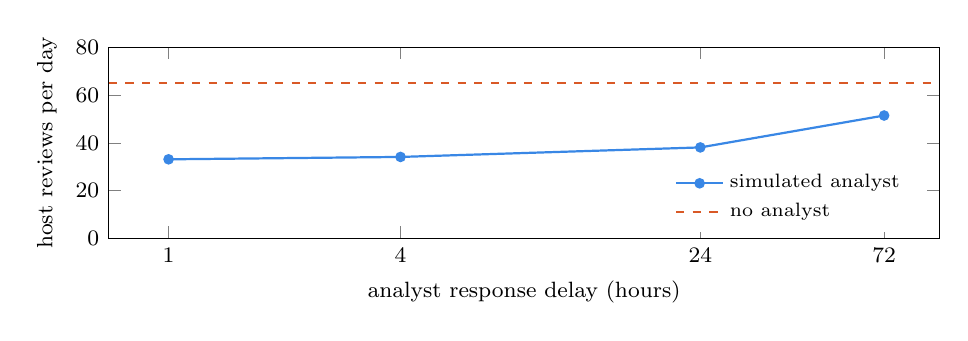
\begin{tikzpicture}
\begin{axis}[width=\columnwidth, height=4.0cm, xmode=log, xmin=0.7, xmax=100, ymin=0, ymax=80,
  xtick=data, log ticks with fixed point, xlabel={analyst response delay (hours)},
  ylabel={host reviews per day}, font=\footnotesize, legend cell align=left, legend pos=south east,
  legend style={font=\scriptsize, draw=none}]
\addplot[cllm, thick, mark=*, mark size=1.5pt] coordinates {(1,33.1) (4,34.1) (24,38.1) (72,51.5)};
\addlegendentry{simulated analyst}
\addplot[ctext, thick, dashed, domain=0.7:100, samples=2] {65.2};
\addlegendentry{no analyst}
\end{axis}
\end{tikzpicture}
\caption{Host reviews per day against the analyst's response delay (C5). At every delay the 72 malicious cases
were raised and the same 400 labelled attack events alerted.}
\label{fig:delay}
\end{figure}

\subsection{C6: asymmetric trust}
We re-scored the same recorded answers under asymmetric trust; these numbers are the asymmetric-trust rows of C1
and C4 (Tables~\ref{tab:text} and~\ref{tab:dedale}). On GUIDE, suppression did not change (4/428, 3/437, 10/437):
those clean alerts were answered only because the model read their clean text, and limiting the model's output
cannot restore what the injected text hid. The rule removed a different effect. Under the acting rule any review
held back an alert's automatic responses, so contamination that triggered a review cancelled a block the trusted
telemetry supported: in 20 of 178 (11.2\%), 18 of 168 (10.7\%) and 21 of 176 (11.9\%) pairs. ERA's own, correct
escalation was the trigger in 17, 18 and 17 of these pairs. Under asymmetric trust the block runs and the review is
added: 0 of 178, 168 and 178 (Fig.~\ref{fig:text}, right). The denominators can grow because a clean alert's block now also runs when its own
hypotheses ask for review. Outcome totals on the development pairs stayed at 532 reviews and 336 automatic
responses. In E1 on DEDALE, 0/72 attack cases were dismissed for every injected text, with and without an analyst;
no pattern was learned and the same 400 events alerted. Reviews per day were 65.2 without and 34.1 with an analyst
whatever the injected text, so the text no longer changes the workload. The cost is the dismissals NCE used to
make; under asymmetric trust it dismissed 0 benign cases, with or without an analyst (C4). Without an analyst the
system reviews 65.2 cases a day instead of 54.8; with one, 34.1 instead of 33.2. On DEDALE, asymmetric trust thus
reviews every case the store has not learned (913 of 913 test cases in the NCE run), and its workload equals that of
NCE off: 65.2 reviews per day, and 34.1 with an analyst (asymmetric-trust rows of C4; NCE off in C4 and C3).

\section{Discussion and Limitations}\label{sec:discussion}

\textbf{Robustness came from structure, not from the model.} On its own the model was easy to mislead: as an
undefended agent it was hijacked on 130 of 439 GUIDE pairs (29.6\%), and in E1 it pointed at the steered host in 30
of 38 injected cases (C1). What kept
injected text from acting was the decision structure around the model, the principle CaMeL~\cite{camel} applies to
agents in general; asymmetric trust turns it into a rule that can be checked case by case.

\textbf{Limits on output do not help where the model is the detector.} GUIDE's 4 of 428 suppressed pairs remain
under asymmetric trust because the model's reading of the clean text was the only thing that raised them. On
DEDALE the store's novelty check raises the cases and the model only adds to them, which is why 0/72 attack cases
were dismissed in E1 on DEDALE. Detection should rest on signals the attacker does not write.

\textbf{Review should be added to automatic containment, not substituted for it.} The containment result (C6) shows
that a correct escalation becomes the attacker's lever when it also pauses a response that trusted evidence already
supports.

\textbf{The analyst is the open channel.} Analysts have to read the evidence, attacker text included, and their
benign verdicts teach the store. C3 shows how far a misled analyst can poison it; unlearning helps only after some
analyst confirms the host, which happened for both attacked hosts in our runs.

\textbf{Limitations.}
\begin{itemize}
\item One testbed dataset with one attack scenario, and labels for 2 attacked Windows clients (the results file's
Limits section). In GUIDE v2,
the entities, evidence text and payloads were generated synthetically.
\item A simulated analyst: an oracle that follows the labels, with independent random mistakes. Real analysts'
errors are likely to cluster on the cases an attacker disguises best, which would likely make the poisoning results
in C3 worse.
\item DEDALE was run with a single model, gemini-3.1-flash-lite; gpt-oss-20b was used on the GUIDE development pairs
only. Each condition ran once; replay reproduces the same numbers on every rebuild, but we did not measure how much
the model's answers vary between runs.
\item The analyst channel: asymmetric trust covers what the LLM's output can cause, not what an analyst decides
after reading attacker text. We also assume the structured sensor fields are not tampered with; an attacker who can
alter them is out of scope.
\item Each free-text field reaches the model cut to 512 characters. On DEDALE the command line exceeds that in 1 of
797 cases, while the raw log line exceeds it in 718 of 856, so attacker text placed late in a raw line never reaches
the model (C4). With asymmetric trust in place, the loss is at most an escalation that does not happen.
\item On GUIDE, where the model is the only detector, contamination still suppressed 4 of 428 responses, with or
without asymmetric trust (C1).
\item Attack activity whose structured pattern also occurs in benign activity stays silent: of the 473 labelled
attack events that raise alerts before any learning, 73 no longer do once the benign weeks are learned (C2). Many
labelled events are of kinds the detectors do not watch.
\item Evasion by mimicry: detection rests on the novelty of patterns built partly from values the attacker chooses
(program names and paths, pipe names, written-file types, PowerShell script text through its hash). An attacker who
copies a learned pattern, for example by naming and placing a binary like a routine program started by its usual
parent, raises no alert; we did not evaluate such deliberate mimicry.
\item Triage runs once per case, on its first alert. Later alerts with the same pattern join the open case without
a new decision, so evidence that arrives later in a case is not reasoned about until a new case opens.
\item No prompt-level defence~\cite{spotlighting,struq} was evaluated as a baseline: the pipeline is compared only
with an undefended triage agent. A comparison with a hardened prompt, in which the untrusted fields are delimited
and declared to be data, was prepared on DEDALE but could not be completed, because the model's API returned only
overload errors (HTTP 503) during the attempts.
\item The host detectors and the open-world rule were chosen on DEDALE itself; E1 injects text only into command
lines; all containment is simulated.
\end{itemize}

\section{Conclusion and Future Work}
AgentSOC proposed combining an LLM's hypotheses with structural checks and risk-ranked responses. Building the
loop and attacking it showed that the dangerous paths run through what the model's output may trigger and what the
store may learn. Learning the benign weeks cut host reviews from 6095.4 to 65.2 per day with the same 400 attack
events alerting (C2); without the gate the store learned 38 attack cases' patterns, and unlearning undid the poisoning a
mistaken analyst caused (C3). Asymmetric trust closed the attacker's route through the model for what the LLM's
output can cause: in E1 on DEDALE, 0/72 attack cases were dismissed whatever text the attacker wrote (C1). Next
steps are the hardened-prompt baseline we prepared but could not complete, evaluation with real analysts, a second
labelled dataset, repeated model runs, and defences for the analyst channel.

\section*{Data and Code Availability}
\todo{repository link}. The recorded LLM answers and the script that rebuilds every number are part of it.

\begin{thebibliography}{99}
\bibitem{agentsoc} J.~Roy and S.~K.~Singh, ``AgentSOC: A multi-layer agentic AI framework for security operations
automation,'' in \emph{Proc. 5th IEEE Int. Conf. on AI in Cybersecurity (ICAIC)}, Houston, TX, USA, 2026,
arXiv:2604.20134.
\bibitem{guide} S.~Freitas, J.~Kalajdjieski, A.~Gharib, and R.~McCann, ``AI-driven guided response for security
operation centers with Microsoft Copilot for Security,'' arXiv:2407.09017, 2024.
\bibitem{dedale} M.~Lanvin and F.~Majorczyk, ``DEDALE: Dataset for evaluating detection of APT among logs and
events,'' Recherche Data Gouv, 2026, doi:10.57745/Y5JLDG.
\bibitem{attack} B.~E.~Strom, A.~Applebaum, D.~P.~Miller, K.~C.~Nickels, A.~G.~Pennington, and C.~B.~Thomas,
``MITRE ATT\&CK: Design and philosophy,'' The MITRE Corporation, Tech. Rep., 2018.
\bibitem{alahmadi} B.~A.~Alahmadi, L.~Axon, and I.~Martinovic, ``99\% false positives: A qualitative study of SOC
analysts' perspectives on security alarms,'' in \emph{Proc. 31st USENIX Security Symp.}, 2022.
\bibitem{perez} F.~Perez and I.~Ribeiro, ``Ignore previous prompt: Attack techniques for language models,'' in
\emph{NeurIPS ML Safety Workshop}, 2022, arXiv:2211.09527.
\bibitem{greshake} K.~Greshake, S.~Abdelnabi, S.~Mishra, C.~Endres, T.~Holz, and M.~Fritz, ``Not what you've signed
up for: Compromising real-world LLM-integrated applications with indirect prompt injection,'' in \emph{Proc. 16th
ACM Workshop on Artificial Intelligence and Security (AISec)}, 2023.
\bibitem{liu} Y.~Liu, Y.~Jia, R.~Geng, J.~Jia, and N.~Z.~Gong, ``Formalizing and benchmarking prompt injection
attacks and defenses,'' in \emph{Proc. 33rd USENIX Security Symp.}, 2024.
\bibitem{spotlighting} K.~Hines, G.~Lopez, M.~Hall, F.~Zarfati, Y.~Zunger, and E.~Kiciman, ``Defending against
indirect prompt injection attacks with spotlighting,'' arXiv:2403.14720, 2024.
\bibitem{struq} S.~Chen, J.~Piet, C.~Sitawarin, and D.~Wagner, ``StruQ: Defending against prompt injection with
structured queries,'' in \emph{Proc. 34th USENIX Security Symp.}, 2025.
\bibitem{camel} E.~Debenedetti \emph{et al.}, ``Defeating prompt injections by design,'' arXiv:2503.18813, 2025.
\bibitem{antidote} B.~I.~P.~Rubinstein, B.~Nelson, L.~Huang, A.~D.~Joseph, S.~Lau, S.~Rao, N.~Taft, and
J.~D.~Tygar, ``ANTIDOTE: Understanding and defending against poisoning of anomaly detectors,'' in \emph{Proc. 9th
ACM SIGCOMM Internet Measurement Conf. (IMC)}, 2009.
\bibitem{agentpoison} Z.~Chen, Z.~Xiang, C.~Xiao, D.~Song, and B.~Li, ``AgentPoison: Red-teaming LLM agents via
poisoning memory or knowledge bases,'' in \emph{Advances in Neural Information Processing Systems (NeurIPS)}, 2024.
\bibitem{poisonedrag} W.~Zou, R.~Geng, B.~Wang, and J.~Jia, ``PoisonedRAG: Knowledge corruption attacks to
retrieval-augmented generation of large language models,'' in \emph{Proc. 34th USENIX Security Symp.}, 2025.
\bibitem{unlearning} Y.~Cao and J.~Yang, ``Towards making systems forget with machine unlearning,'' in \emph{Proc.
IEEE Symp. on Security and Privacy (S\&P)}, 2015.
\end{thebibliography}

\end{document}
